\documentclass{article}
\usepackage{tabularx,fullpage,url}
\usepackage[top=1in, bottom=1in, left=.5in, right=.75in]{geometry}
\usepackage{amsmath,amssymb,graphicx,amsthm,xparse, color, mathrsfs} 
\usepackage{ epstopdf, fullpage}

\usepackage{xifthen}

\newcommand{\mypagebreak}{\begin{center}
		\noindent\makebox[\linewidth]{\rule{7.5in}{1pt}}
	\end{center}}
\bibliographystyle{siam}
\newcommand{\minimize}[1]{\underset{#1}{\text{minimize}}}
\newcommand{\mini}[1]{\underset{#1}{\text{min}}}
\newcommand{\argmin}[1]{\underset{#1}{\text{argmin}}}
\newcommand{\st}{\mathrm{subject to}}
\newcommand{\rank}{\mathbf{rank}}
\newcommand{\epi}{\mathbf{epi}}

\newcommand{\diag}{\mathbf{diag}}
\newcommand{\mb}{\mathbf}
\newcommand{\R}{\mathbb R}
\newcommand{\mle}{\mathbf{MLE}}
\newcommand{\map}{\mathbf{MAP}}
\newcommand{\bE}{\mathbb E}
\newcommand{\mL}{\mathcal L}
\newcommand{\mH}{\mathcal H}
\newcommand{\mN}{\mathcal N}
\newcommand{\mD}{\mathcal D}
\newcommand{\mC}{\mathcal C}

\newcommand{\mS}{\mathcal S}
\newcommand{\mB}{\mathcal B}
\newcommand{\tr}{\mathbf{tr}}
\newcommand{\mrm}{\mathrm}
\newcommand{\proj}{\mathbf{proj}}
\newcommand{\prox}{\mathbf{prox}}
\newcommand{\sign}{\mathbf{sign}}
\newcommand{\range}{\mathbf{range}}
\newcommand{\vnull}{\mathbf{null}}
\newcommand{\pr}{\mathbf{Pr}}
\newcommand{\find}{\mathbf{find}}
\newcommand{\argmax}[1]{\underset{#1}{\mathrm{argmax}}}
\newcommand{\subjto}{\mathrm{subject~to}}

\newcommand{\bmat}{\left[\begin{matrix}}
\newcommand{\emat}{\end{matrix}\right]}

\newcommand{\red}[1]{{\color{red}#1}}

\newcommand{\gray}[1]{\textcolor{lightgray}{#1}}


\newcommand{\ifequals}[3]{\ifthenelse{\equal{#1}{#2}}{#3}{}}
\newcommand{\case}[2]{#1 #2} 
\newenvironment{switch}[1]{\renewcommand{\case}{\ifequals{#1}}}{}

\newcommand{\duedate}[1]{
    \begin{switch}{#1}
        \case{1}{Monday, Sept. 14}
        \case{2}{Wednesday, Sept. 23}
        \case{3}{Monday, Oct. 5}
        \case{4}{Wednesday, Oct. 28}
        \case{5}{Monday, Nov. 9}
        \case{6}{Wednesday, Nov. 18}
    \end{switch}
}


\newcommand{\homeworknumber}{2}

\newcommand{\showsolution}[1]{\textbf{Ans.} \;#1}
\newcommand{\showsolutionpts}[2]{\textbf{Ans. (#1 pts)} \;#2}


\begin{document}
{\Large\textbf{CSE 512: Homework  \hfill
Due \duedate{\homeworknumber} }}


\mypagebreak

\begin{enumerate}
\item Consider the problem 
\begin{equation}
\minimize{x} \quad \overbrace{\underbrace{\frac{1}{2}\|Ax-b\|_2^2}_{=:f(x)} + \frac{\rho}{2}\|x\|_2^2}^{F(x)}
\label{eq:hw2:linreg}
\end{equation}
where $A\in \R^{m\times n}$ and $n > m$.
\begin{enumerate}
\item Is the function $f(x) = \frac{1}{2}\|Ax-b\|_2^2$ $L$-smooth? Is it $\mu$- strongly convex? If not, why? If so, what are the value of $L$ and $\mu$?

\showsolutionpts{0.5}{
The Hessian is $\nabla^2 f(x) = A^TA$. Then $L = \lambda_{\max}(A^TA)$ and $\mu = \lambda_{\min}(A^TA)$. Since $n > m$, then $\mu = 0$, and the function is not strongly convex. However, since $L$ is a finite number, the function is $L$ -smooth.
}

\item Is the function $F(x) = f(x) + \frac{\rho}{2}\|x\|_2^2$ $L$-smooth or $\mu$-strongly convex? If not, why? If so, what are the values of $L$ and $\mu$?

\showsolutionpts{0.5}{
The trick here is to see that 
\[
\nabla^2 F(x) = A^TA + \rho I
\]
and furthermore 
\[
\lambda_{\max}(A^TA + \rho I) = \lambda_{\max}(A^TA) + \rho, \qquad \lambda_{\min}(A^TA + \rho I) = \lambda_{\min}(A^TA) + \rho.
\]
Again, $L = \lambda_{\max}(A^TA + \rho I)$ is finite, so $F$ is $L$-smooth, and now since $\mu = \rho > 0$, it is also strongly convex.
}

\item \textbf{Exponential convergence.} Consider $b = 0$ and $\rho > 0$.
Show that in this case, then gradient descent with step size $ \alpha < 1/L$ on \eqref{eq:hw2:linreg} converges with \emph{exponential complexity}, e.g. for some constant $c$, the error $f(x^{(t)}) - f(x^*) = O(c^t)$.


\showsolutionpts{0.5}{
It is sufficient here to cite previous responses and say that a strongly convex function has exponential convergence.

If you were to prove it, here is an example proof.


First, note that for this scenario, the optimal objective value is $F(x) = f(x) = 0$, and can be achieved by $x^*= 0$. 
If $b = 0$ then gradient descent repeats the iteration scheme 
\begin{eqnarray*}
x^{(t+1)} &=& x^{(t)} - \alpha A^TA  x^{(t)} - \alpha \rho  x^{(t)}\\
&=&(I-\alpha A^TA-\alpha \rho I)x^{(t)}\\
&=&(I-\alpha A^TA-\alpha \rho I)^t x^{(1)}.
\end{eqnarray*}

Take the eigenvalue decomposition $A^TA = U \diag(\lambda) U^T$, and  do a change of variables $z^{(t)} := U^Tx^{(t)}$. Then the recurrence simplifies to
\[
z^{(t)} = (I-\alpha \diag(\lambda)- \alpha \rho I)^t z^{(1)}
\]
and in fact each step is requires an element-wise multiplication. So, we try to set up a contraction, since we know that $z^* = U^Tx^* = 0$ is a solution:
\[
\|z^{(t)}\|_\infty \leq (1 - \alpha \underbrace{\lambda_{\min}}_{=0} - \alpha \rho)^t\|z^{(1)}\|_\infty.
\]
Taking in particular $\alpha < 1/L$ gives
\[
\|z^{(t)}\|_\infty \leq \left(1-\frac{\rho}{L}\right)^t\|z^{(1)}\|_\infty.
\]
Note also that in general, for any vector $z\in \R^n$, $\|z\|_2 \leq \sqrt{d}\|z\|_\infty$, and furthermore, since $U$ is orthonormal, 
\[
\|z^{(t)}\|_2 = \|Ux^{(t)}\|_2 = \|x^{(t)}\|_2.
\]
Finally, 
\begin{eqnarray*}
f(x^{(t)}) - \underbrace{f^*}_{=0} &=& \frac{1}{2}\|Ax^{(t)}\|_2^2 + \frac{\rho}{2}\|x^{(t)}\|_2^2 \\
&=& \frac{1}{2}\|\Lambda z^{(t)}\|_2^2 + \frac{\rho}{2}\|z^{(t)}\|_2^2\\
&\leq & (\lambda_{\max} + \rho)\frac{1}{2}\|z^{(t)}\|_2^2 = O(\beta c^{(t)})
\end{eqnarray*}
for 
\[
\beta =  (\lambda_{\max} + \rho)n\|z^{(1)}\|_\infty, \qquad c = \left(1-\frac{\rho}{L}\right).
\]
}



\item \textbf{Nullspace component. (2.5pts)} Now consider $A = \bmat 1 & 1 \\ 1 & 1 \emat$,  $b = \bmat 1 \\ -1\emat $, and $\rho = 0$. 

\begin{enumerate}
\item Recall that for any vector $x$, from the linear decomposition theorem, we can uniquely write 
\[
x = u + v, \qquad u \in \vnull(A), \quad v\in \range(A^T).
\]
We will denote the operation of pulling out the nullspace component of $x$ as $u = \proj_{\vnull(A)}(x)$. 
Suppose that we run gradient descent for \eqref{eq:hw2:linreg}, starting at $x^{(0)} = \bmat 0 \\ 0 \emat$. After $t$ iterations, what is $\proj_{\vnull(A)}(x^{(t)})$? Why?


\showsolution{
First, the term $b$ is a red herring, and doesn't really matter. In particular, suppose that for any $t$, we form the decomposition $x^{(t)} = u^{(t)} + v^{(t)}$ where $u^{(t)} = \proj_{\vnull(A)}(x^{(t)})$. Then 
\[
x^{(t+1)} = x^{(t)} - \underbrace{\alpha A^T(Ax^{(t)}-b)}_{g}.
\]
Then for \emph{any} $b$, $\proj_{\vnull(A)}(g) = 0$, in particular because $g$ is in the range of $A^T$. You can prove this in more detail by taking the SVD of $A = U\Sigma V^T$, and therefore 
\[
\proj_{\vnull(A)}(g) = (I - VV^T)g \overset{g=A^Tw}{=} (I-VV^T)A^Tw=(V-V)\Sigma^T U^Tw = 0.
\]
In other words, if $\proj_{\vnull(A)}(x^{(0)}) = 0$, then $\proj_{\vnull(A)}(x^{(t)}) = 0$ for \emph{any} $t>0$.

}

\item Now suppose that $x^{(0)} = \bmat 1 \\ -1 \emat$. After $t$ iterations, what is $\proj_{\vnull(A)}(x^{(t)})$? Why?

\showsolution{
Using the same logic as in the previous part,  by linearity of projections, 
\[
\proj_{\vnull(A)}(x^{(t)}) = \proj_{\vnull(A)}(x^{(t-1)}) -\underbrace{\proj_{\vnull(A)}(\alpha A^T(Ax^{(t-1)}-b)) }_{=0} = \proj_{\vnull(A)}(x^{(0)}).
\]
Since $x^{(0)} = \bmat 1 \\ -1 \emat \in \vnull(A)$, then $\proj_{\vnull(A)}(x^{(t)}) = x^{(0)}$ for all $t$.
}

\item Now suppose that $\rho = 1$. For both cases of initial values, after $t$ iterations, what is $\proj_{\vnull(A)}(x^{(t)})$? Why?

\showsolution{
With regularization, the iteration scheme at each step now includes a multiplicative shrinking of $x^{(t)}$ at each step; namely,
\[
x^{(t+1)} = x^{(t)} - \underbrace{\alpha  A^T(Ax^{(t)}-b)}_{\in \vnull(A)} - \alpha x^{(t)}.
\]
So, now, at each step, 
\[
\proj_{\vnull(A)}(x^{(t)}) = (1-\alpha )\proj_{\vnull(A)}(x^{(t-1)}) = (1-\alpha )^t \proj_{\vnull(A)}(x^{(0)}).
\]
If $x^{(0)} = \bmat 0 \\ 0 \emat$, then this nullspace component is still 0 for all $t$. If $x^{(0)} = \bmat 1 \\ -1 \emat \in \vnull(A)$, then this component is $(1-\alpha)^t\bmat 1 \\ -1 \emat$, which for $\alpha < 1$, shrinks at each step.
}

\end{enumerate}

\end{enumerate}


\item \textbf{Convex functions} 

\begin{enumerate}
\item Recall the objective function in logistic regression
\[
f(\theta) = -\frac{1}{m}\sum_{i=1}^m \log(\sigma(y_ix_i^T\theta)), \qquad \sigma(s) = \frac{1}{1 + \exp(-s)}.
\]
Show that $f(\theta)$ is convex.

\showsolutionpts{0.5}{
Since $f$ is twice differentiable, the easiest way to do this is to look at the Hessian and show that it is positive semidefinite. 
\[
\nabla^2 f(\theta) = Z^TDZ
\]
where each row of $Z$ is $y_ix_i$, and $D = \diag(d_1,...,d_m)$ for $d_i = \sigma(y_ix_i^T\theta)(1-\sigma(y_ix_i^T\theta)) \geq 0$.
Then for any $w$, $w^T\nabla^2 f(\theta)w = \|D^{1/2}Zw\|_2^2\geq 0$, so the Hessian is always positive semidefinite.
}

\item In matrix factorization, we attempt to characterize a matrix $R\in \R^{m\times n}$ in terms of low-rank factors  $R \approx UV^T$, where $U\in \R^{m\times r}$ and $V\in \R^{n\times r}$. Take $r = 1$.  (Note that $\rank(R) > 1$ in general.)
Show that
\[
f(u,v) = \frac{1}{2}\|R-uv^T\|_F^2
\]
is nonconvex.



\showsolutionpts{0.5}{
Gradient 
\[
\nabla_u f(u,v) = (uv^T-R)v, \qquad \nabla_v f(u,v) = (vu^T-R^T)u
\]
Hessian 
\[
\nabla^2 f(u,v) = \bmat \nabla_{uu}^2 f(u,v) & \nabla_{uv}^2 f(u,v) \\ \nabla_{vu}^2 f(u,v) & \nabla_{vv}^2 f(u,v)\emat 
= \bmat 
v^Tv I & 2uv^T - R\\ 2 vu^T-R^T & u^Tu I
\emat
\]
Without loss of generality, assume that the maximum singular value of $R$ is 2. We can always renormalize all the terms here to make this true. Writing the singular value decomposition of $R$ as 
\[
R = \sum_{i=1}^{\min\{m,n\}}\sigma_i u_iv_i^T, \qquad \sigma_1 = 2
\]
we pick $u = u_2$ and $v = v_2$. Then 
\[
\nabla^2 f(u_2,v_2) =  \bmat 
 I & 2u_2v_2^T - R\\ 2 v_2u_2^T-R^T & u_2^Tu_2 I
\emat.
\]    
To show that the Hessian is not positive semidefinite at this point, it suffices to find any $w$ where $w^T \nabla^2 f (u_2,v_2)w < 0$. Pick $w = \bmat u_1 \\ v_1 \emat$. Then 
\[
w^T \nabla^2 f (u_2,v_2)w = u_1^Tu_1 + v_1^Tv_1 - 2 u_1^TRv_1 = 1 + 1 - 2 \sigma_1 = -2.
\]
}
\end{enumerate}

\item \textbf{Convex sets} 

\begin{enumerate}
\item \textbf{Norm balls.} Consider $\|x\|$ any norm. Show that the norm properties dictate that the \emph{norm balls}, defined as 
\[
\mB_r = \{x : \|x\|\leq r\}
\]
are always convex sets. Show that for any $r > 0$, the complement set 
\[
\bar\mB_r = \{x : \|x\| > r\}
\]
is nonconvex.

\showsolutionpts{0.5}{
Positive homogeneity and subadditivity give you the convexity of $\mB_r$.
Suppose that $\|x\|\leq r$ and $\|y\|\leq r$; this, $x, y \in \mB_r$. Then  for any $0 \leq \theta \leq 1$, 
\[
\|\theta x + (1-\theta)y\| \overset{\text{subadditivity}}{\leq} \|\theta x\| + \|(1-\theta) y\| \overset{\text{pos. homogeneity}}{=}\theta\underbrace{\|x\|}_{\leq r} + (1-\theta)\underbrace{\|y\|}_{\leq r} \leq r.
\]
Thus, $\theta x + (1-\theta)y \in \mB_r$.

To show the nonconvexity of $\bar\mB_r$, it suffices to pick $x = -y$, for some $\|x\|>r$. Then $\|y\|>r$ by symmetry, but picking $\theta = 1/2$, then $\|\theta x+(1-\theta) y\|=0<r$ for any $r > 0$. 
}


\item \textbf{Level sets.} For a function $f:\R^d \to \R$, we define the \emph{level sets} as 
\[
\mS_r = \{x : f(x) \leq r\}.
\]
Show that if $f$ is convex, then all of its level sets $\mS_r$ are convex. Is the opposite true? (If a function has only convex level sets, is it necessarily convex?)

\showsolutionpts{0.5}{
The first part follows very similarly to the proof for convex norm balls. In particular, suppose that $x\in \mS_r$ and $y\in \mS_r$, which implies that $f(x) \leq r$ and $f(y) \leq r$. Then by convexity, for any $0 \leq \theta \leq 1$,
\[
f(\theta x + (1-\theta) y) \leq \theta f(x) + (1-\theta) f(y) \leq r
\]
and therefore $\theta x + (1-\theta) y \in \mS_r$. 


The opposite is not necessarily true, as is shown by the existence of \emph{quasi-convex functions}. In particular, consider the function $f(x) = \sqrt{|x|}$. This function has all convex level sets ($\mS_r = [-\sqrt{r},\sqrt{r}]$ convex intervals), but picking $x = 0$, $y = 1$, and $\theta = 1/2$, we see that 
\[
f(\theta x + (1-\theta) y) = f(1/2) = 1/\sqrt{2} > 1/2 =\theta f(x) + (1-\theta) f(y).
\]
}

\end{enumerate}




\item Consider the hard margin SVM 
\begin{equation}
\minimize{\theta\in \R^n} \quad \frac{1}{2}\|\theta\|_2^2 \qquad \subjto \quad y_ix_i^T\theta \geq 1, \quad  i = 1,...,m
\label{eq:hw2:svm}
\end{equation}
We would like to solve \eqref{eq:hw2:svm} using projected gradient descent. However, projecting on this constraint set (a halfspace) 
\[
\mH = \{\theta : y_ix_i^T\theta \geq 1, \quad \forall i\}
\]
is extremely nontrivial. (One possible way to do it is to use Dykstra's projection on the intersection of convex sets, where you iteratively project on the halfspace determined by each $i$, and use proper scaling. However, this takes a long time to converge, so we won't go there.)

We do this by first introducing \emph{slack variables} $s_i$, and rewriting \eqref{eq:hw2:svm} equivalently as
\begin{equation}
\begin{array}{ll}
\minimize{\theta\in \R^n, s\in \R^m} & \frac{1}{2}\|\theta\|_2^2 \\
 \subjto & y_ix_i^T\theta = 1 + s_i, \quad  i = 1,...,m\\
 & s \geq 0
 \end{array}
\label{eq:hw2:svm2}
\end{equation}
This problem is still a bit hard to solve, because the simultaneous projection on the affine constraint $y_ix_i^T\theta = 1 + s_i$ and the halfspace constraint $s \geq 0$ is as hard as projecting on $\mH$. So, we will use a trick by transforming a constraint to a penalty. Specifically, we want to find a function $\phi(s)$ which is large when $s$ violates the nonnegativity constraint, and 0 otherwise. We pick 
\[
\phi(s) = \frac{1}{2}\sum_{i=1}^m (\max\{-s_i, 0\})^2
\]
and we consider the revised problem 
\begin{equation}
\begin{array}{ll}
\minimize{\theta\in \R^n, s\in \R^m} & \frac{1}{2}\|\theta\|_2^2 + \rho \phi(s) \\
 \subjto & y_ix_i^T\theta = 1 + s_i, \quad  i = 1,...,m.
 \end{array}
\label{eq:hw2:svm3}
\end{equation}
\begin{enumerate}



\item For a fixed value of $\rho$, what is the gradient of the objective function of \eqref{eq:hw2:svm3}? Is it $L$-smooth, and if so, what is the value of $L$?

\showsolutionpts{1}{
The gradient of $f$ can be written as 
\[
\nabla f(\theta, s) = \bmat \nabla_\theta f(\theta,s)\\ \nabla_s f(\theta,s) \emat = \bmat \theta \\ \rho \min\{s_i,0\} \emat.
\]
Since the gradient $\nabla_\theta f(\theta,s)$ doesn't depend on $s$, and $\nabla_s f(\theta,s)$ doesn't depend on $\theta$, the problem is \emph{separable}, and in fact we can consider the $L$-smoothness of each gradient block separately. First, 
\[
\|\nabla_\theta f(\theta_1,s_1) - \nabla_\theta f(\theta_2,s_2) \|_2^2 = \|\theta_1-\theta_2\|_2^2 \leq \|\theta_1-\theta_2\|_2^2 + \|s_1-s_2\|_2^2
\]
so $\nabla_\theta f(\theta,s)$ is 1-Lipschitz continuous.

Similarly,
\[
\|\nabla_s f(\theta_1,s_1) - \nabla_s f(\theta_2,s_2) \|_2^2 \leq \rho^2\|s_1-s_2\|_2^2 \leq \rho^2(\|\theta_1-\theta_2\|_2^2 + \|s_1-s_2\|_2^2)
\]
so $\nabla_s f(\theta,s)$ is $\rho$-Lipschitz continuous.

Overall, we get that $\nabla f$ is $\max\{1,\rho\}$-Lipschitz continuous, so $f$ is $\max\{1,\rho\}$-smooth.
}


\item The least squares solution given by most solvers is also the \emph{least norm solution}. That is, if the linear system $A\theta = b$ is solvable (there exists at least one solution) then the command $\texttt{solve(A,b)}$ gives the unique solution to the optimization problem 
\[
\minimize{\theta} \quad \|\theta\|_2 \qquad \subjto \quad A\theta = b.
\]

Use this information to describe the steps to computing the projection onto the feasible set in \eqref{eq:hw2:svm3}. That is, given any $\hat \theta$, $\hat s$, show how to return the solution to
\begin{equation}
\minimize{\theta,s} \quad \|\theta-\hat \theta\|_2^2 + \|s-\hat s\|_2^2 \qquad \subjto \quad y_ix_i^T\theta = 1 + s_i, \;  i = 1,...,m.
\label{eq:hw2:projsvm}
\end{equation}

\showsolutionpts{1}{
We first rewrite some things to make this problem look more approachable. We concatenate all our variables together
\[
\hat w = \bmat \hat \theta\\\hat s\emat
\]
and write out the linear system in a more familiar way:
\[
 A = \bmat Z & -I\emat, \quad b = \mb 1.
\]
Now \eqref{eq:hw2:projsvm} can be rewritten as 
\begin{equation}
\minimize{w} \quad \|w-\hat w\|_2^2 \qquad \subjto \quad Aw=b.
\label{eq:hw2:projsvm:1}
\end{equation}
The next step is to simply use a change of variables. We define $\tilde w = w - \hat w$, and then rewrite \eqref{eq:hw2:projsvm:1} as
\begin{equation}
\minimize{w} \quad \|\tilde w\|_2^2 \qquad \subjto \quad A\tilde w=b -A \hat w.
\label{eq:hw2:projsvm:2}
\end{equation}
Now, \eqref{eq:hw2:projsvm:2} is just a min-norm least squares problem! We can solve this using simply
\texttt{solve(A, b-np.dot(A, what))}, or \texttt{solve(A, b-A* what)}!

Then $w$ can be recovered by taking $w = \tilde w + \hat w$, and the projected $\theta$, $s$ can be extracted from $w = \bmat \theta \\ s\emat$.
}




\item \textbf{Coding (2pts)} 
\begin{itemize}
\item Download \texttt{arrhythmia.zip} and take a look at the three files inside. The original data is loaded in \texttt{arrhythmia.data} which is a csv file, with 279 features followed by a class label. A description of each feature and label is given in \texttt{arrhythmia.names}. 
Take a look at it, and understand what it is saying.

\item The file \texttt{arrhythmia.mat} contains the data from \texttt{arrhythmia.data} loaded and organized, so that you have 
$x_i \in \R^{279}$ containing the $n = 279$ features  and $y_i \in \{1,2,\cdots,15\}$ indicating the patient's diognosis. The matrix $X$ and vector $y$ are packed so that
\[
X = \bmat x_1^T \\ \vdots \\x_m^T\emat \in \R^{m\times n} \text{ and } y = \bmat y_1 \\ \vdots \\ y_m \emat \in \R^m.
\]
We want to convert this multiclass classification problem to a binary classification problem, so adjust $y$ so that $y = 1$ means the patient is normal, and $y = -1$ means the patient is anything but normal. Comment on the class balancing; e.g., does it look like each class has enough ``data representatives"?


\item \textbf{Train/test split} To eliminate randomness, I have given you two index vectors: \texttt{idx\_train} and \texttt{idx\_test}, which randomly form a 60/40 train/test split. Later, when we discuss cross validation, we will see that you actually need to make these splits multiple times, to convince yourself that you are not overfitting. For now, we will just use these. 

Form a train and test data and label set using these indices. In python, your code should look like 

\begin{verbatim}
Xtrain = X[idx_train,:]
ytrain = y[idx_train]
Xtest = X[idx_test,:]
ytest = y[idx_test]
\end{verbatim}

and in MATLAB,

\begin{verbatim}
Xtrain = X(idx_train,:);
ytrain = y(idx_train);
Xtest = X(idx_test,:);
ytest = y(idx_test);
\end{verbatim}



\item \textbf{Normalizing} Now we will use a more ``standardized" normalization scheme, which is what is recommended if you don't really know anything special about your data. If we were medical experts, we might try something fancier, but for this exercise let's just do the simplest thing: de-meaning, followed by de-variancing. 

As before, first calculate the mean data vector over the training data
\[
x_{\text{mean}} = \frac{1}{m_{\text{train}}} \sum_{i=1}^{m_\text{train}} x_i
\]
and remove this offset from the train and test data.

Next, calculate the mean standard deviation over the training data:
\[
x_{\text{std}}[k] = \frac{1}{m_{\text{train}}} \sqrt{\sum_{i=1}^{m_\text{train}} x_i[k]^2}
\]
This can be done with the built in \texttt{std} function in MATLAB or Python.
Remove this multiplicatively from the train and test data, e.g.
\[
x_i[k] \leftarrow x_i[k] /x_{\text{std}}[k] 
\]

Now we're ready to go!

\end{itemize}

\begin{enumerate}
\item Solve the hard margin SVM reformulation in \eqref{eq:hw2:svm3}, sweeping $\rho = 10^{-4}, 10^{-2}, 1., 10^2$. Use a zero initialization as before, and $1/L$ as your stepsize with $L$ as calculated in part (a). Run for 1000 iterations.

Plot the margin value and the penalty $\phi(s)$ for the train set, and the train and test misclassificatition errors. Do this for $t = 1,...,1000$. Report also these final values.

\showsolution{
Final values:

\begin{tabular}{r|cccc}
$\rho$& margin & $\phi(s)$ & train misclass rate & test misclass rate \\\hline
$10^{-4}$& 8.761 &104.703 &0.265 &0.267\\
$10^{-2}$& 1.971 &64.090& 0.147& 0.233\\
$1$& 0.219 &13.7833 &0.015& 0.328\\
$10^2$& 0.078 &0.038 &0.0 &0.361
\end{tabular}

\begin{center}
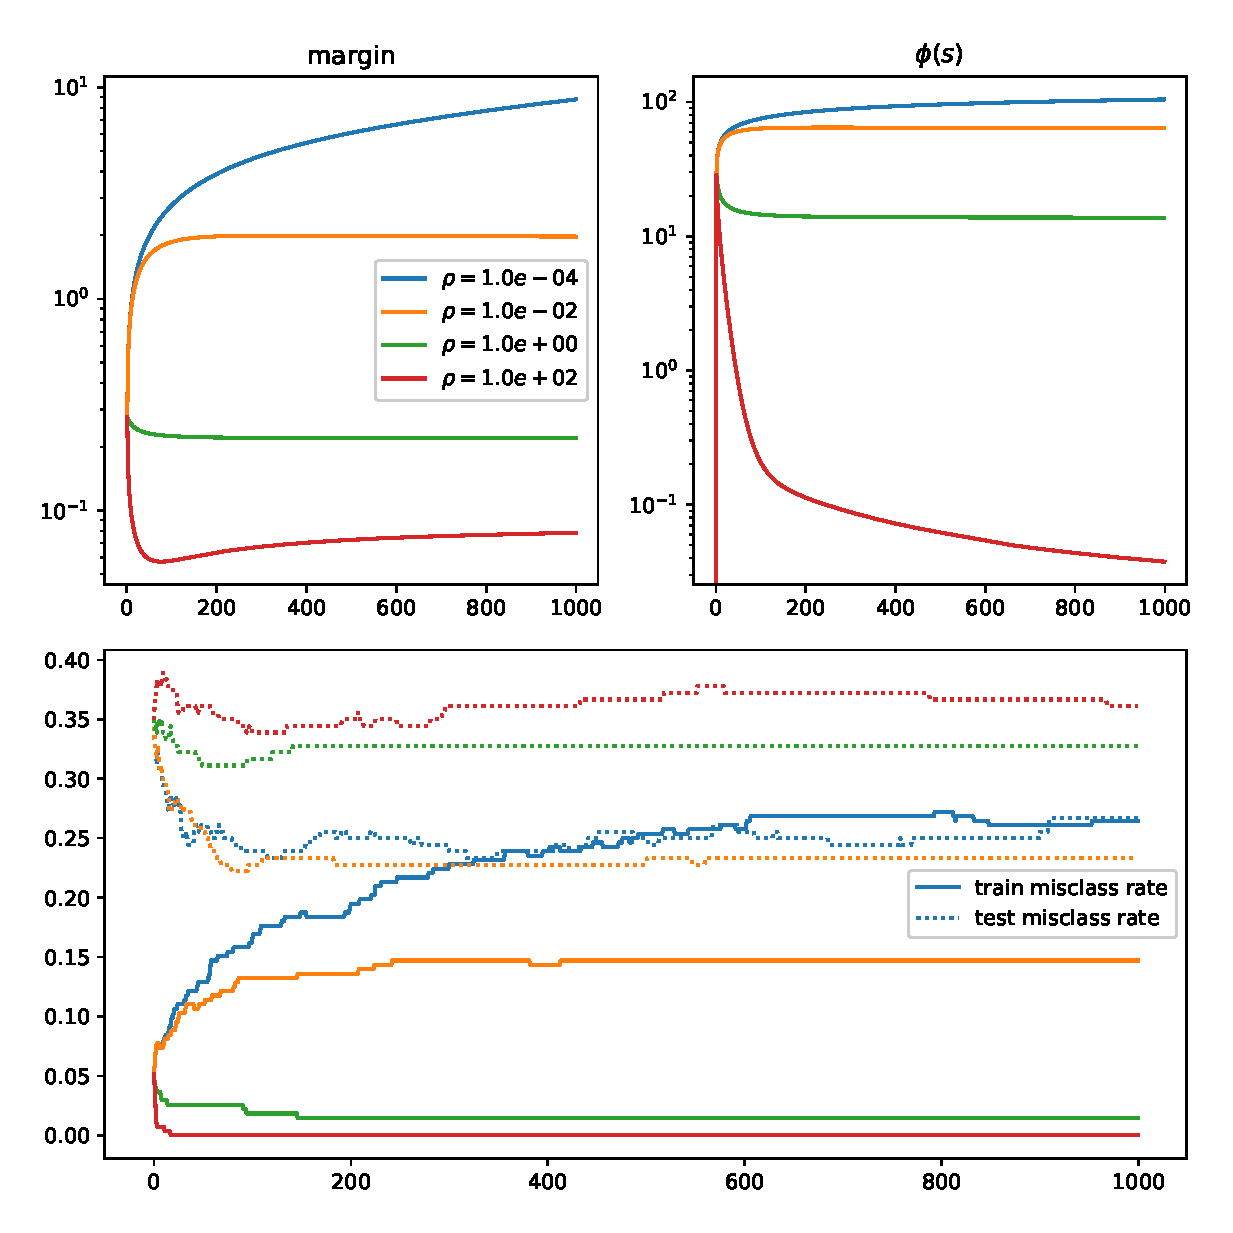
\includegraphics[width=4in]{figs/hw2_svm.eps}
\end{center}
}

\item Is the data separable?  Is this a reasonable approach for constrained optimization, given large enough $\rho$?

\showsolution{Yes, the data is separable. With  a large enough $\rho$, we are able to achieve $\phi(s) = 0$, which shows that the feasible set in \eqref{eq:hw2:projsvm:2} is attainable.}

\item Comment a bit on the \emph{test} misclassification rate for varying values of $\rho$.

\showsolution{
While a large enough $\rho$ ensures that \eqref{eq:hw2:svm3} (the formulation we solve) is equivalent to \eqref{eq:hw2:svm2} (the actual hard margin SVM), it seems to worsen test performance. There seems to be a sweet spot, at about $\rho = 0.01$, where both performance of train and test misclassification rate seem reasonable, but if we increase $\rho$ too much then the test misclassification rate begins to degrade.

Actually, this is an example of overfitting. Hard margin SVM in itself is asking a bit too much of this dataset; even though the data \emph{is} separable, by forcing it this way we are creating a hyperplane that is a bit too tuned to the train set, and not that effective on the test set. While we can use cross validation (discussed later) to pick the best value of $\rho$, the conclusion I would draw from this experiment is to simply use the soft margin SVM instead, which uses a \emph{hinge penalty function} for $\phi$. 
}

\end{enumerate}



\end{enumerate}



\end{enumerate}


\newpage

\section*{Challenge!}

This challenge will  look at two interesting extensions of the SVM problem.
\begin{enumerate}



\item \textbf{Projected gradient descent} 
Consider the convex constrained optimization problem 
\begin{equation}
\minimize{\theta} \quad f(\theta) \qquad \subjto \quad \theta \in \mC
\label{eq:hw2:constrained}
\end{equation}
where $f:\R^d\to\R$ is a convex function and $\mC$ is a convex set. The \emph{normal cone} to $\mC$ at a given point $\theta$ is defined as  the set of points orthogonal to the tangent cone of $\mC$ at $\theta$; explicitly, it is 
\[
\mN_\mC(\theta) := \{g : g^T(\theta' - \theta) \leq 0, \quad \forall \theta' \in \mC\}.
\]
Recall that in \emph{unconstrained} optimization, an optimality condition for convex optimization is that $\theta^*$ minimizes $f(\theta)$ if and only if $0 = \nabla f(\theta^*)$. In \emph{constrained} optimization, the optimality condition is a bit more complicated:
\[
\theta^* \text{ optimizes } \eqref{eq:hw2:constrained} \iff -\nabla f(\theta^*) \in \mN_\mC(\theta^*).
\]
\begin{enumerate}
\item Show that  if $\theta^*$ is in the interior of $\mC$, then this reduces to the condition of $0 = \nabla f(\theta^*)$. 
(We say that $\theta$ is in the interior of $\mC$ if  for any vector $v$ we can find $\epsilon > 0$ small enough such that $\theta + \epsilon v\in \mC$.)

\showsolution{
This follows from the observation that if $\theta$ is in the interior of $\mC$ then $\mN_\mC(\theta) = \{0\}$. Specifically, take $\theta = \theta^* + \epsilon v$ for any $v:\|v\|_2=1$. Then $\theta^*\in \mN_\mC$ implies $\epsilon \nabla f(x^*)^Tv = 0$ for all $v$. Therefore $\nabla f(x^*) = 0$.

}

\item Recall the \emph{projected gradient descent} method for solving \eqref{eq:hw2:constrained} at each iteration computes 
\[
\theta^{(t+1)} = \proj_{\mC}(\theta^{(t)} - \alpha \nabla f(\theta^{(t)}))
\]
for some step size $\alpha > 0$. Show that when this method is stationary, then optimality is reached. That is, any $\alpha > 0$,
\[
\theta^* = \proj_\mC(\theta^* - \alpha \nabla f(\theta^* ))\quad \iff \quad -\nabla f(\theta^*) \in \mN_\mC(\theta^*).
\]

\showsolution{
Let's define condition (A) as $\theta^* = \proj_{\mC}(\theta^*-\alpha\nabla f(\theta^*))$, and condition (B) as $-\nabla f(\theta^*)\in \mN_\mC(\theta^*)$. We wish to show that (A) $\iff$ (B).

\begin{eqnarray*}
(A) &\iff & \theta^* = \argmin{\theta\in \mC} \|\theta^*-\alpha \nabla f(\theta^*)-\theta\|_2^2\\
&\overset{\text{argmin = it's a minimum}}{\iff}& \|\theta^*-\alpha \nabla f(\theta^*)-\theta^*\|_2^2 \leq \|\theta^*-\alpha \nabla f(\theta^*)-\theta\|_2^2, \quad \forall \theta \in \mC\\
&\overset{\text{simplify}}{\iff} & \alpha^2 \|\nabla f(\theta^*)\|_2^2 \leq \alpha^2 \|\nabla f(\theta^*)\|_2^2 + \|\theta^*-\theta\|_2^2 - \alpha \nabla f(\theta^*)^T(\theta^*-\theta) , \quad \forall \theta \in \mC\\
&\overset{\text{simplify}}{\iff} & -\nabla f(\theta^*)^T(\theta-\theta^*) \leq  \frac{\|\theta^*-\theta\|_2^2 }{\alpha}, \quad \forall \theta \in \mC.
\end{eqnarray*} 
Since this is true for all $\alpha > 0$, for all $\theta\in \mC$ arbitrarily close to $\theta^*$, then we can safety say that (A) $\iff$ (B).

}

\end{enumerate}


\item \textbf{Kaczmarz method.} In question 4 we found a way to find a separation in our dataset by solving some projection problems at each iteration. But, what if the number of training samples were very large? Then computing the projection at each step is extremely burdensome.

Von Neumann in the 1949 figured out that a way to project on the intersection of hyperplanes is to just alternatingly project on each hyperplane. That is, if I want to find some $\theta$ where $A\theta = b$, then I could break down $A$ and $b$ as 
\[
A = \bmat A_1 \\ A_2 \\ \vdots \\ A_K \emat, \qquad b = \bmat b_1 \\ b_2 \\ \vdots \\ v_K\emat
\]
and we simply need to find $\theta$ where 
\[
A_i \theta = b_i \qquad \text{ for } i = 1,...,K.
\]
Then using von Neumann's approach, we would simply pick any $\theta^{(0)}$, and alternatingly do
\[
\theta^{(t+1)} = \proj_{\mC_i} (\theta^{(t)})
\]
where $\mC_i = \{\theta : A_i \theta = b_i\}$. Then, for $i$ large enough, $\theta^{(i)}$ will converge to the true intersection of hyperplanes.

This principle, when applied to this data separation problem,  is also sometimes known as Kaczmarz' method. Specifically, we are going to break down our data matrix so that we only operate on one sample at a time. Unlike von Neumann's approach, however, we are only going to make a few passes through the data. This doesn't ensure full feasibility, but the hypothesis is that we get something reasonable nonetheless.

\begin{enumerate}
\item Describe the projection method on feasibility of a \emph{single} data sample: e.g. given $\hat \theta$,  how would we solve
\[
\minimize{\theta} \quad \|\theta - \hat \theta\|_2^2 \qquad \subjto \quad y_ix_i^T\theta  = 1?
\]
Use the linear decomposition theorem to give an \emph{explicit} solution, e.g. using matrix-vector multiplications only, and no matrix inverses. (One scalar inverse should be used.)

Note that we are ignoring the slack variable in this approach, and forcing an equality rather than inequality.

\showsolution{
From previous bits of the homework, we know that our goal is to solve the min-norm least squares problem 
\[
\minimize{\tilde \theta} \quad \|\tilde \theta\|_2^2  \qquad \subjto \quad z^T\tilde \theta = 1-z^T\hat \theta
\]
for $z =  y_ix_i $.

From the linear decomposition theorem, we know that we can uniquely write $\tilde \theta = \tilde u + \tilde v$ where 
\[
\tilde u = \proj_{\vnull(z^T)}(\tilde \theta), \qquad \tilde v = \proj_{\range(z)}(\tilde \theta).
\]
Explicitly, from previous notes, we know that in fact, if we had $\tilde w$, then
\[
\tilde v = \frac{z^T\tilde \theta}{z^Tz} z, \qquad \tilde u = \tilde w - \tilde v.
\]
We could plug this into our optimization, getting the equivalent reformulation:
\[
\minimize{\tilde u, \; \tilde v} \quad \|\tilde u\|_2^2 + \|\tilde v\|_2^2 \qquad \subjto \quad \underbrace{z^T\tilde u}_{=0} + z^T\tilde v = 1-z^T\hat \theta
\]
which shows us that in fact, $\tilde u$ does not participate in the constraints at all; therefore $\tilde u = 0$ minimizes the objective and is attained. Now our problem reduces to 
\[
\minimize{\tilde v} \quad  \|\tilde v\|_2^2 \qquad \subjto \quad z^T\tilde v = 1-z^T\hat \theta
\]
where our desired $\tilde \theta = \tilde v$. But wait!  the term $z^T\tilde \theta$ is constrained! Therefore 
\[
\tilde \theta = \tilde v = \frac{z^T\tilde v}{z^Tz} z = \frac{1-z^T\hat \theta}{z^Tz} z.
\]
Overall, this gets us 
\[
\theta = \frac{1-z^T\hat \theta}{z^Tz} z + \hat \theta.
\]
}

\item Initialize at $\theta^{(0)} = 0$. Randomly permute the training data samples. Then, taking 5 passes through the training data (permuting the data at each pass) where for each data sample, you project the current iterate  on the feasible set for each data sample. After the 5 passes, pass, plot the margin size, infeasibility ($\sum_i \max\{1-y_ix_i^T\theta,0\}$), and misclassification rate over the test and train set. 
Do this for 5 separate random permutations.


\showsolution{

\begin{center}
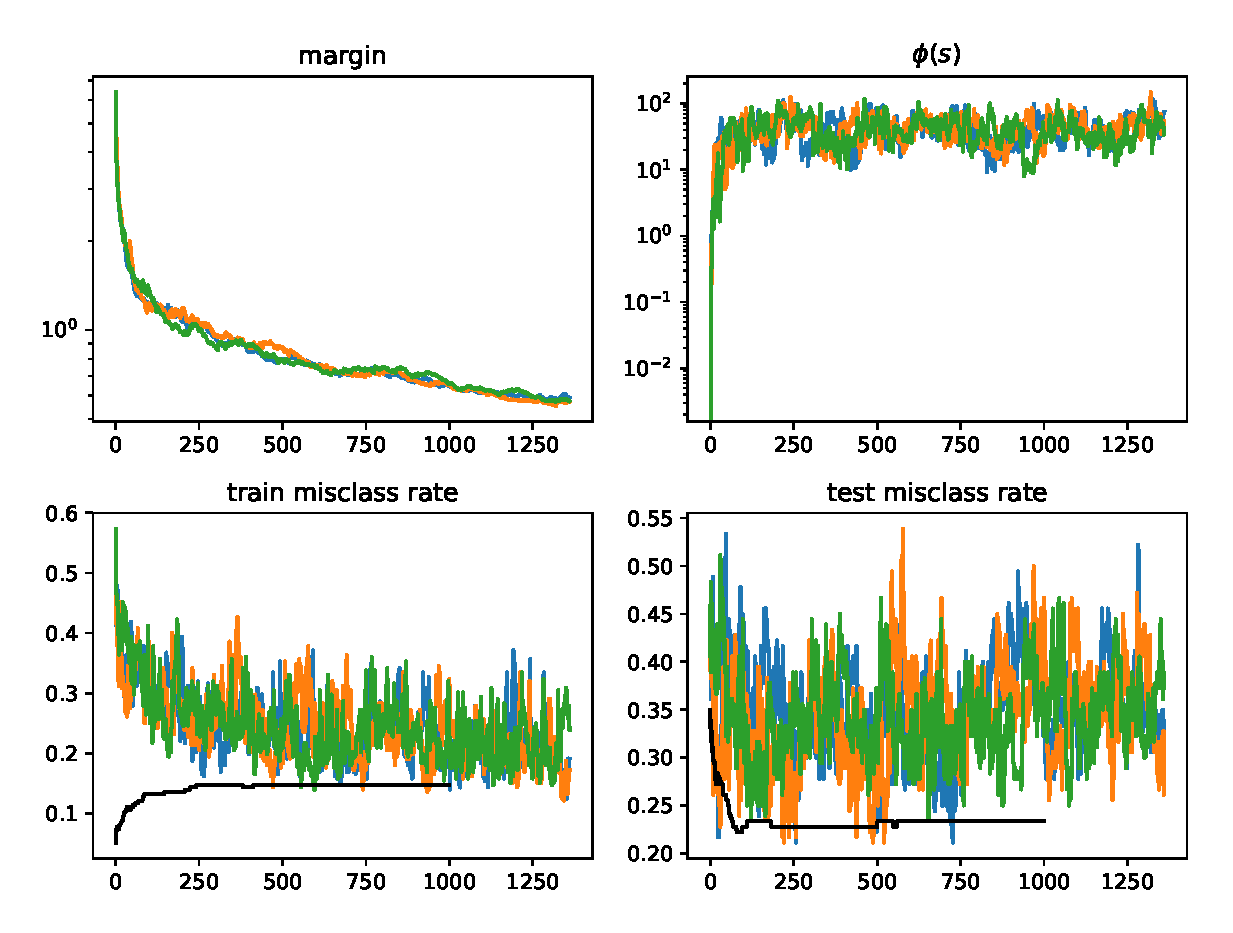
\includegraphics[width=4in]{figs/hw2_kaczmarz.eps}
\end{center}

In black is the comparison against the modified hard-margin SVM approach, using $\rho = 0.01$. (Best parameter from previous part.)
}


\item Comment on what you see. Is this a viable method? How is its generalization behavior? Compare it with the behavior from the SVM approach.

\showsolution{
The thing I want to point out here is that here, each iteration touches only \emph{one data sample}, whereas in the previous approach, with the SVM, at each iteration we did a projection on the \emph{entire data set}. Yet, we are clearly able to do quite a bit with the training misclassification rate, and the test misclassification rate does go down a bit, though not as well as the best case $\rho$ in the modified hard margin SVM. Overall, I would rate this method as ``not bad, but not as good as full on SVM, but much more scalable to big data."
}

\end{enumerate}


\end{enumerate}

\end{document}